\documentclass[11pt]{article}

\usepackage[a4paper,margin=27mm]{geometry}
\usepackage[T1]{fontenc}
\usepackage[utf8]{inputenc}
% Times-like text and math as in the preceding study's manuscript when newtx is installed; otherwise mathptmx.
\usepackage{amsmath}
\usepackage{amsthm}
\IfFileExists{newtxtext.sty}{\usepackage{newtxtext}\usepackage{newtxmath}}{\usepackage{mathptmx}}
\usepackage{microtype}
\usepackage{booktabs}
\usepackage{tabularx}
\usepackage{graphicx}
\usepackage{caption}
\usepackage{enumitem}
\usepackage{xcolor}
\usepackage{seqsplit}
\usepackage{tikz}
\usetikzlibrary{positioning,arrows.meta}
\usepackage[hidelinks]{hyperref}

\microtypesetup{protrusion=false}
\setlength{\emergencystretch}{3em}
\captionsetup{font=small,labelfont=bf}
\renewcommand{\topfraction}{0.9}
\renewcommand{\textfraction}{0.07}
\renewcommand{\floatpagefraction}{0.85}
\setlist[itemize]{leftmargin=*,topsep=3pt,itemsep=1pt}
\setlist[enumerate]{leftmargin=*,topsep=3pt,itemsep=2pt}

\theoremstyle{plain}
\newtheorem{proposition}{Proposition}
\newtheorem{observation}{Observation}
\theoremstyle{definition}
\newtheorem{definition}{Definition}

\newcommand{\argine}{\textsc{Argine}}
\newcommand{\code}[1]{\texttt{\seqsplit{#1}}}
\newcommand{\hsh}[1]{\texttt{\seqsplit{#1}}}
\newcommand{\klow}{\kappa_{\mathrm{low}}}
\newcommand{\gate}[1]{{\itshape\fontsize{6}{7}\selectfont #1}}

\title{\textbf{Predictive Structure Is Not Retention Value:\\
A Prospective Falsification of Prediction-Led Expert\\
Retention in Memory-Constrained Mixture-of-Experts Inference}}
\author{sennape}
\date{November 2026}

\begin{document}
\maketitle

\begin{abstract}
A preceding study established that expert routing in Qwen3-30B-A3B-Q4\_K\_M contains causal predictive structure. The present study asks whether that information can be converted into useful real-runtime retention value when expert weights must be served from a fixed memory budget. We report a sequence of prospectively specified tests on one consumer host. First, the original runtime realization did not consume policy events with the reference semantics: it issued 144 policy calls per decode token where the reference defines 48, because each physical expert-tensor operation was treated as an independent semantic update; after correction, runtime conformance passed. Second, the predictor and bookkeeping path has substantial cost: a standalone microbenchmark attributes 123.68~$\mu$s per call (5.94~ms/token at 48 calls) to the predictor, and in situ the policy counters explain the observed overhead ($\rho=0.9024$, 95\% Fieller CI $[0.8760, 0.9287]$). Third, in an 18-block paired runtime experiment at the primary 1.5~GiB budget, the corrected predictive policy was slower than its baseline by 15.83~ms/token (95\% CI $[10.46, 21.19]$; $-2.93\%$ throughput). Fourth, offline counterfactuals on an extracted event stream that reproduces the runtime mechanism counters exactly show that a clairvoyant Belady-style comparator removes 40.673\% of baseline misses, that a zero-cost shield protecting only the experts of the event being served obtains 2.43$\times$ the byte benefit of the original predictive mechanism, and that the best tested causal next-use predictive eviction policy captures 8.79\% of the oracle miss-byte headroom. Its conservative gross value, 8.11~ms/token, fails a prospectively frozen 10~ms/token viability floor before any policy-computation cost is charged. Within the tested regime, predictive structure in expert routing did not translate into economically useful retention control. The study does not establish how much of the oracle headroom is causally recoverable, and it does not test prefetch, overlap, scheduling, admission control or oracle-distilled policies.
\end{abstract}

%=====================================================================
\section{Introduction}
\label{sec:intro}

Mixture-of-experts (MoE) models activate a small subset of experts per token~\cite{shazeer2017sparsely,fedus2022switch}. When the full set of expert weights does not fit in fast memory, inference systems keep a resident subset and load the rest on demand, and a long line of systems work exploits routing behaviour through caching, offloading or prediction~\cite{eliseev2023offloading,xue2025moeinfinity,kamahori2025fiddler,liu2026survey}. A natural hypothesis is that if expert usage is predictable, a retention policy that keeps the experts likely to be used soon should reduce misses and therefore wall time.

A preceding study~\cite{argine2paper} established the first half of that chain for one model and runtime: routing contains measurable layer-local and transition structure, a strictly causal predictor beats trivial baselines on sealed held-out data, and a predictor-driven reactive policy reduces miss bytes in validated offline replay. It also reported that the same policy did not improve real decode throughput. The present study investigates the second half of the chain: \emph{can the predictive expert information established by the preceding study be converted into useful real-runtime retention value?}

The answer we report is \emph{no, within the tested regime}. The contribution is not the negative answer alone but the decomposition of why: (i) the first runtime realization was semantically non-equivalent to the reference; (ii) after correction, the predictor's bookkeeping cost is measured and attributed; (iii) the corrected policy causes a net runtime loss; (iv) offline counterfactuals show that the original mechanism captured almost none of the available clairvoyant headroom and that its small effect is reproduced without prediction; and (v) moving the prediction to the future eviction decision raises the captured headroom roughly 38-fold relative to the original mechanism, yet still fails a prospectively frozen economic floor even at zero computation cost. Every stage's classification or kill rule was frozen before its data were analysed. Figure~\ref{fig:chain} summarizes the chain; Table~\ref{tab:stages} lists the stages and their outcomes.

The preceding study is not contradicted. Its predictive results concern forecasting quality and replay-level retention on its frozen stream, and they remain valid. The present study measures a different quantity: whether the information is worth its cost when it controls retention in a real runtime.

\begin{figure}[t]
\centering
% Figure 1: evidence chain of the present study (reader-facing stage names; each box lists its frozen gate).
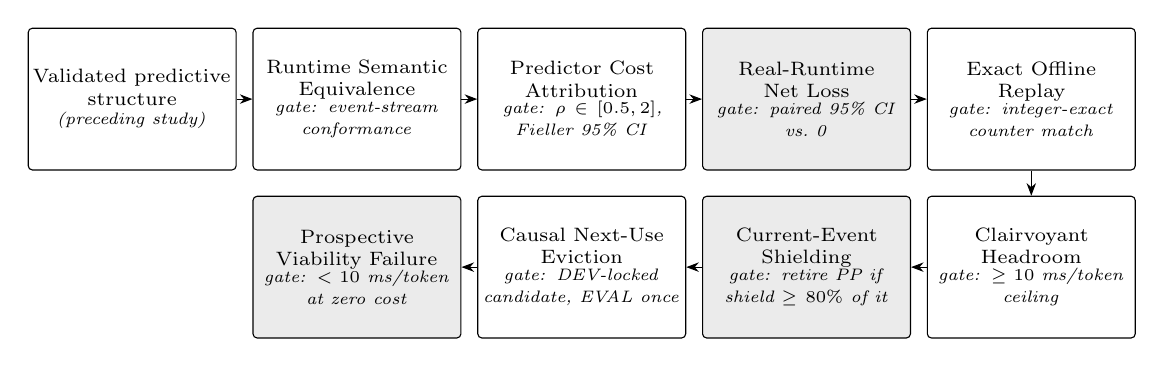
\begin{tikzpicture}[
  node distance=3.2mm and 2.0mm,
  box/.style={draw, rounded corners=1.5pt, align=center, font=\scriptsize, text width=25mm, minimum height=18mm, inner sep=2pt},
  neg/.style={box, fill=black!8},
  arr/.style={-{Stealth[length=1.6mm]}, thin}]
\node[box] (n1) {Validated predictive\\structure\\[-1pt]\gate{(preceding study)}};
\node[box, right=of n1] (n2) {Runtime Semantic\\Equivalence\\[-1pt]\gate{gate: event-stream\\conformance}};
\node[box, right=of n2] (n3) {Predictor Cost\\Attribution\\[-1pt]\gate{gate: $\rho\in[0.5,2]$,\\Fieller 95\% CI}};
\node[neg, right=of n3] (n4) {Real-Runtime\\Net Loss\\[-1pt]\gate{gate: paired 95\% CI\\vs.\ 0}};
\node[box, right=of n4] (n5) {Exact Offline\\Replay\\[-1pt]\gate{gate: integer-exact\\counter match}};
\node[box, below=of n5] (n6) {Clairvoyant\\Headroom\\[-1pt]\gate{gate: $\ge 10$ ms/token\\ceiling}};
\node[neg, left=of n6] (n7) {Current-Event\\Shielding\\[-1pt]\gate{gate: retire PP if\\shield $\ge 80\%$ of it}};
\node[box, left=of n7] (n8) {Causal Next-Use\\Eviction\\[-1pt]\gate{gate: DEV-locked\\candidate, EVAL once}};
\node[neg, left=of n8] (n9) {Prospective\\Viability Failure\\[-1pt]\gate{gate: $<10$ ms/token\\at zero cost}};
\draw[arr] (n1) -- (n2); \draw[arr] (n2) -- (n3); \draw[arr] (n3) -- (n4); \draw[arr] (n4) -- (n5);
\draw[arr] (n5) -- (n6); \draw[arr] (n6) -- (n7); \draw[arr] (n7) -- (n8); \draw[arr] (n8) -- (n9);
\end{tikzpicture}

\caption{Evidence chain of the present study. Each box is one stage, with its frozen gate in italics; shaded boxes are negative outcomes. Every gate was frozen prospectively, and no stage's classification rule was changed after its result was seen.}
\label{fig:chain}
\end{figure}

\begin{table}[t]
\centering
\caption{Stages of the present study and their outcomes. Every outcome was decided by a rule frozen before the data were analysed; the exact frozen classification labels and repository identifiers are given in Appendix~\ref{app:prov}.}
\label{tab:stages}
\small
\begin{tabularx}{\linewidth}{>{\raggedright\arraybackslash}p{0.27\linewidth}>{\raggedright\arraybackslash}X>{\raggedright\arraybackslash}p{0.22\linewidth}}
\toprule
Stage & Scientific question & Outcome \\
\midrule
Runtime Semantic Equivalence & Does the corrected runtime realize the reference event semantics? & Semantic conformance: PASS \\
Predictor Cost Attribution & Does direct policy bookkeeping explain the sham-over-baseline overhead? & Bookkeeping cost: EXPLAINED \\
Real-Runtime Retention Evaluation & Does the real predictive retention policy beat the baseline policy end to end? & Real-runtime evaluation: NET LOSS \\
Offline Replay Fidelity & Does offline replay reproduce the runtime mechanism counters? & Offline replay: FIDELITY PASS \\
Clairvoyant Retention Headroom & Is there clairvoyant retention headroom worth $\ge 10$ ms/token? & Clairvoyant headroom: HEADROOM PRESENT \\
Current-Event Shielding & Is the effect of the original predictive mechanism reproduced by a zero-cost current-event shield? & Original predictive mechanism: RETIRED \\
Causal Next-Use Eviction & Does causal next-use eviction clear the zero-cost floor? & Causal predictive retention: VIABILITY FAIL \\
\midrule
Overall & Can validated predictive information be converted into useful retention value? & NEGATIVE RESULT IN TESTED REGIME \\
\bottomrule
\end{tabularx}
\end{table}

%=====================================================================
\section{Background and Preceding Study}
\label{sec:background}

\paragraph{System.} \argine{} serves Qwen3-30B-A3B-Q4\_K\_M~\cite{qwen3technicalreport} through a modified llama.cpp runtime~\cite{gerganov2023llamacpp} whose expert store keeps a byte-budgeted resident set of (layer, expert) objects: 48 MoE layers, 128 experts per layer, top-$k=8$ routing, and two expert byte sizes (about 2.65 and 3.06~MB). A miss loads the expert from the store before computation; every policy admits on demand.

\paragraph{Baseline.} The baseline retention policy \code{b\_selected} is aged frequency (score decay 0.999 per access, aging interval 1 at 1.5~GiB), selected in the preceding study on development data and frozen. Victims minimize (aged score, last reference, layer, expert).

\paragraph{Predictor and predicted\_protect.} The frozen causal predictor \code{decayed\_transition} (decay 0.99) predicts, after each event of a layer, the top-$k$ experts of that layer's next event. In the preceding study it beat trivial baselines at horizon 1 (mean recall@$k$ 0.449817 vs.\ 0.401473, $+12.04\%$)~\cite{argine2paper}. The retention mechanism \code{predicted\_protect} (PP) evicts as \code{b\_selected} except that residents of the current layer whose expert is in that layer's predicted set are shielded, with a total fallback. A sham arm (\code{predicted\_protect\_sham}) performs identical predictive bookkeeping but chooses victims exactly as \code{b\_selected}.

\paragraph{Preceding study.} The preceding study~\cite{argine2paper} proceeded from oracle feasibility to real-runtime validation in thirteen stages (Table~\ref{tab:prev}). It first validated an offline replay against runtime telemetry and measured, across memory budgets, the gap between a causal baseline and a clairvoyant Belady-style comparator, a comparator-relative margin that is not a proven bound on causal recovery. It then characterized routing (concentration, transition structure, reuse and working-set locality, workload dependence), froze a prediction benchmark, selected and confirmed a causal predictor, showed in replay that a predictor-driven reactive policy reduced miss bytes, and finally tested that policy in the real runtime, where no throughput gain was found. The present study begins at that last result.

\begin{table}[t]
\centering
\caption{Progression of the preceding study. Repository identifiers of the stages are given in Appendix~\ref{app:prov}.}
\label{tab:prev}
\footnotesize
\begin{tabularx}{\linewidth}{r>{\raggedright\arraybackslash}p{0.25\linewidth}>{\raggedright\arraybackslash}X>{\raggedright\arraybackslash}X}
\toprule
 & Stage & Scientific question & Outcome relevant here \\
\midrule
1 & Oracle Trace Contract and Replay Validation & Does offline replay of a runtime trace agree with runtime telemetry? & Zero event disagreements on the measured coding trace. \\
2 & Oracle vs Retention Baselines & How far is a causal LRU baseline from a clairvoyant comparator? & At 4~GiB the comparator has 58.59\% fewer miss bytes. \\
3 & Expert-Memory Budget Sensitivity & How does that gap depend on the memory budget? & 44.11\% at 1.5~GiB, 70.66\% at 8~GiB, none at 16~GiB. \\
4 & Recoverable-Margin Analysis & Is the gap a recoverable margin? & Gap rises then collapses at full residency; not a proven bound on causal recovery. \\
5 & Expert Frequency and Concentration & Is layer-local routing non-uniform? & Yes (median effective expert fraction 0.514). \\
6 & Routing Transition Structure & Does the previous routing state inform the next? & Yes (median same-layer NMI 0.099, positive in every layer). \\
7 & Reuse Distance and Working-Set Structure & Is short-horizon reuse stronger than chance? & Yes (immediate reuse 0.426 vs.\ 0.187 under a shuffled null). \\
8 & Routing Drift and Workload Dependence & Does routing change more across workloads than over time? & Cross-workload divergence exceeds temporal drift ($2.21\times$). \\
9 & Prediction Benchmark & Which causal baselines set the bar for prediction? & Benchmark contract frozen; development tournament run. \\
10 & Causal Working-Set Predictor & Does the selected causal predictor beat trivial baselines on sealed data? & Yes at horizon 1 (recall@$k$ 0.449817 vs.\ 0.401473, $+12.04\%$). \\
11 & Retention Feasibility Bridge & Can predictions reduce miss bytes in prospective replay? & Positive. \\
12 & Prediction-Driven Retention & Does the predictor-driven reactive policy reduce miss bytes in confirmatory replay? & Yes at 4~GiB (72 of 72 cells). \\
13 & Real-Runtime Decode Throughput & Does that policy raise real decode throughput? & No improvement at 4~GiB; later found inconclusive because of the event-semantics mismatch (Section~\ref{sec:semantics}). \\
\bottomrule
\end{tabularx}
\end{table}

\paragraph{Handoff.} The preceding study's real-runtime validation reported no throughput improvement at 4~GiB ($-0.171721$ tokens/s; frozen outcome: fail)~\cite{argine2paper}. A later audit (Section~\ref{sec:semantics}) found that the runtime realization did not consume policy events with the reference semantics and classified that runtime validation as inconclusive rather than as a test of the reference policy. The present study therefore begins by establishing runtime equivalence.

%=====================================================================
\section{Research Question and Method}
\label{sec:method}

\paragraph{Question.} Can the predictive expert information established by the preceding study be converted into useful real-runtime retention value? The scope is prediction-led retention; the present study is not a general search over memory-management policies.

\begin{definition}[Semantic policy event]
One semantic event is one (forward pass, MoE layer) pair together with the union of experts requested by that layer in that pass. The reference semantics issue exactly one policy update per semantic event; decode passes are those with index $\ge 2$ (event index $\ge 96$), giving 512 decode tokens per run.
\end{definition}

\paragraph{Discipline.} Each stage froze its protocol, endpoints and classification rule before acquisition or analysis, recorded a SHA-256 freeze over its artifacts, and was committed separately (Appendix~\ref{app:prov}). Runtime experiments used a fixed sample size with no optional stopping; offline analyses used integer counters and exact fractions; candidate selection used DEV data only and EVAL was scored once.

\paragraph{Workload and identity.} All runtime and replay results use the frozen coding workload (context 4096, 512 generated tokens, seed 42, temperature 0, top-$k$ 1), the frozen model and store files, and a frozen runtime binary; launches were admitted only if the output token digest matched the frozen digest and exactly 24{,}672 policy events were recorded.

\paragraph{Economic conversion.} To express replay miss bytes in wall time we use the association measured between the 1.5 and 8~GiB budgets of the real-runtime evaluation,
\begin{equation}
\kappa = \frac{T_A(1.5\,\mathrm{GiB}) - T_A(8\,\mathrm{GiB})}{B_A(1.5\,\mathrm{GiB}) - B_A(8\,\mathrm{GiB})} = 0.7584~\mathrm{ms/MB},\qquad \klow = \kappa/2 = 0.3792~\mathrm{ms/MB},
\label{eq:kappa}
\end{equation}
where $T_A$ is baseline decode ms/token and $B_A$ is baseline decode miss MB/token. $\kappa$ is a two-point association, not a causal per-byte law; halving it is a pre-registered conservative choice. For a policy $c$ with decode miss bytes per token $B_c$, the conservative gross value at zero policy cost and its share of the oracle headroom are
\begin{align}
V(c) &= \klow\,(B_A - B_c) \quad [\mathrm{ms/token}], \label{eq:value}\\
H(c) &= \frac{B_A - B_c}{B_A - B_{\mathrm{Bel}}}, \label{eq:capture}
\end{align}
with $B$ in MB/token and $B_{\mathrm{Bel}}$ the Belady-style comparator of Section~\ref{sec:headroom}.

%=====================================================================
\section{Runtime Semantic Equivalence}
\label{sec:semantics}

\subsection{Original Mismatch}
An offline audit of the runtime event stream found that the runtime invoked the policy once per \texttt{MUL\_MAT\_ID} node (gate, up and down projections), that is, three updates with identical expert sets per (pass, layer): 144 policy calls per decode token instead of 48, and 74{,}016 recorded events against 24{,}672 semantic events in a 4~GiB trace. The C++ predictor reproduced the reference exactly on the logged stream; the divergence was in the event stream itself. The consequences follow directly from the update rule: predictor history, transition counts and per-event decay advanced three times per semantic event, so the effective per-event decay was the cube of the frozen value; \code{b\_selected}'s per-access aging was likewise accelerated; and bookkeeping calls tripled. The audit classified the preceding study's replay results as unaffected and the earlier runtime validation as inconclusive.

\subsection{Semantic Correction}
The correction separates two operations that the original runtime had conflated: the \emph{semantic policy update}, now issued once per (pass, layer) over the union expert set, and the \emph{physical expert-store ensure}, which still occurs for every tensor operation that needs a resident expert.

\subsection{Conformance}
Three traced real-model launches (baseline and sham at 4~GiB, baseline at 8~GiB) each recorded 24{,}672 policy events over 514 passes with no missing or duplicate events, matched the frozen output token digest, and showed zero budget violations; the sham's victim sequence equalled \code{b\_selected}'s event for event. Semantic conformance therefore passed. This establishes equivalence of the realized event stream; it does not by itself establish any performance property.

%=====================================================================
\section{Predictor Cost Attribution}
\label{sec:cost}

\subsection{Microbenchmark}
A standalone C++ microbenchmark of the decision path on the evaluation host (Intel Core i5-1340P, Windows, MSVC \code{/O2 /arch:AVX2}) measured mean per-call costs of 8.80~$\mu$s for \code{b\_selected}, 132.48~$\mu$s for the sham and 134.28~$\mu$s for the full policy. The predictor component (sham minus baseline) is 123.68~$\mu$s per call, or 5.94~ms/token at 48 semantic calls per token. The dominant work is algorithmic: the decayed-transition prediction is recomputed densely per event (hash probes, exponentiation and a 128-way sort) although only a small part of its state changes per event.

\subsection{End-to-End Attribution}
The attribution test asked whether in-situ policy bookkeeping accounts for the measured sham-over-baseline wall overhead, with a pre-registered rule: \emph{explained} if and only if the 95\% Fieller interval for $\rho = O/\Pi$ is bounded and inside $[0.5, 2.0]$, where $O$ is the wall overhead (sham minus baseline) and $\Pi$ the in-situ policy-time contrast. In 20 ABBA blocks (80 launches, 8~GiB), $O = 17.466$~ms/token and $\Pi = 19.354$~ms/token, giving $\rho = 0.9024$ with 95\% Fieller CI $[0.8760, 0.9287]$: the overhead is classified as explained. In situ, the predictor path costs 3.26$\times$ its microbenchmark estimate. These costs are specific to the tested runtime, host and configuration.

%=====================================================================
\section{Real-Runtime Retention Evaluation}
\label{sec:runtime}

\subsection{Protocol}
The evaluation compared three arms: A (\code{b\_selected}), S (sham: full predictive bookkeeping, baseline victims) and P (\code{predicted\_protect}). The primary endpoint is decode wall ms/token from server timings over 512 tokens. Estimands are block-level contrasts of 2-launch arm means: $\Delta_{\mathrm{cost}} = S-A$, $\Delta_{\mathrm{ret}} = P-S$ and $\Delta_{\mathrm{net}} = P-A$. The frozen decision rule classifies \textsc{net loss} if the lower bound of the two-sided 95\% $t$ interval of $\Delta_{\mathrm{net}}$ exceeds 0, \textsc{net win} if the upper bound is below 0, and inconclusive otherwise. The schedule had 18 blocks at 1.5~GiB (primary) and 6 at 8~GiB (descriptive negative control), one uncounted warmup per budget, 146 physical and 144 counted launches, a fixed $N$ and no optional stopping. A pre-registered amendment dropped 4~GiB timing before acquisition.

\begin{table}[t]
\centering
\caption{Real-runtime retention evaluation results (decode wall ms/token, 512 tokens; lower is better). Arm rows: per-launch mean, standard deviation and mean tokens/s. Contrast rows: mean over blocks of paired 2-launch arm means, two-sided 95\% $t$ interval. The 8~GiB budget is a descriptive negative control.}
\label{tab:runtime}
\small
\begin{tabular}{llrrrr}
\toprule
Budget & Arm / contrast & $n$ & ms/token & sd or 95\% CI & tok/s \\
\midrule
1.5 GiB (primary) & A (b\_selected) & 36 & 526.97 & 15.19 & 1.8992 \\
 & S (predicted\_protect\_sham) & 36 & 541.56 & 13.25 & 1.8476 \\
 & P (predicted\_protect) & 36 & 542.80 & 13.76 & 1.8435 \\
 & $S-A$ (cost) & 18 blocks & 14.59 & [9.87, 19.31] & \\
 & $P-S$ (retention) & 18 blocks & 1.24 & [$-$2.84, 5.32] & \\
 & $P-A$ (net) & 18 blocks & 15.83 & [10.46, 21.19] & \\
\midrule
8 GiB (control) & A (b\_selected) & 12 & 116.47 & 1.70 & 8.5873 \\
 & S (predicted\_protect\_sham) & 12 & 136.14 & 2.18 & 7.3469 \\
 & P (predicted\_protect) & 12 & 136.60 & 1.83 & 7.3220 \\
 & $S-A$ (cost) & 6 blocks & 19.67 & [17.68, 21.66] & \\
 & $P-S$ (retention) & 6 blocks & 0.45 & [$-$1.25, 2.16] & \\
 & $P-A$ (net) & 6 blocks & 20.12 & [17.87, 22.38] & \\
\bottomrule
\end{tabular}
\end{table}


\subsection{Primary Result}
At 1.5~GiB (Table~\ref{tab:runtime}, Figure~\ref{fig:runtime}), A ran at 526.97~ms/token (1.8992 tok/s), S at 541.56 and P at 542.80~ms/token. The bookkeeping cost $S-A$ was $+14.59$~ms/token (95\% CI $[9.87, 19.31]$); the retention effect $P-S$ was $+1.24$~ms/token with an interval containing zero ($[-2.84, 5.32]$); the net contrast $P-A$ was $+15.83$~ms/token (95\% CI $[10.46, 21.19]$), a $-2.93\%$ throughput change. The frozen rule classifies the result as \textsc{net loss}: the corrected predictive policy did not recover its own cost.

\subsection{Negative Control}
At 8~GiB the resident set is large and retention has little to act on. The control shows the same pattern with larger bookkeeping cost ($S-A = +19.67$~ms/token, $[17.68, 21.66]$) and no detectable retention effect ($P-S = +0.45$, $[-1.25, 2.16]$), consistent with bookkeeping cost and no retention benefit.

\begin{figure}[t]
\centering
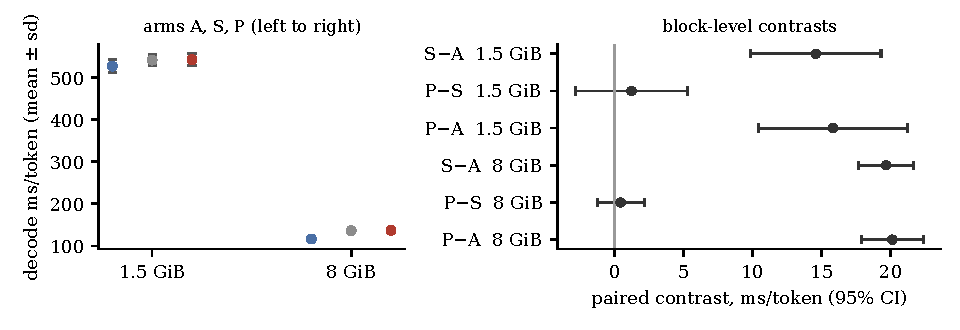
\includegraphics[width=\linewidth]{figures/fig3_runtime.pdf}
\caption{Real-runtime results. Left: arm means $\pm$ per-launch sd (A, S, P). Right: block-level paired contrasts with two-sided 95\% $t$ intervals (18 blocks at 1.5~GiB, 6 at 8~GiB).}
\label{fig:runtime}
\end{figure}

%=====================================================================
\section{Prospective Falsification of Predictive Retention}
\label{sec:why}

This sequence, the Prospective Predictive-Retention Falsification, asked whether the net loss was a consequence of the particular mechanism and its placement rather than of prediction-led retention as such. It was run offline, with kill rules K0--K5 frozen in a protocol written before any of its numbers were computed.

\subsection{Offline Replay Fidelity}
The canonical event stream (514 passes, 24{,}672 semantic events, token digest identical to the real-runtime evaluation) was extracted from the semantic-conformance traces; the three traces yield identical streams. Replaying the frozen Python reference policies on it at 1.5~GiB reproduces the runtime mechanism counters integer-exactly: 106{,}491 decode misses (207.990~misses/token) for A and 106{,}390 (207.793) for PP. The fidelity check passes. Counterfactual policies can therefore be evaluated offline on this stream.

\subsection{Clairvoyant Retention Headroom}
\label{sec:headroom}
The comparator is the repository's historical Belady-style global policy: on a miss it evicts the resident whose next use is farthest in the future, never evicts members of the event being served, and admits on demand. Because events are multi-key and byte sizes differ slightly by layer, it is a strong reference but is not proven optimal. At 1.5~GiB it reduces decode misses from 207.990 to 123.395 per token ($-40.673\%$) and miss bytes by 40.653\%, i.e.\ 43{,}313 misses and 124{,}509{,}708{,}288 bytes (243.18~MB/token) of headroom. By Eq.~\eqref{eq:value} this is worth at most 92.216~ms/token at $\klow$, so the headroom criterion (K1) is met: the failure of PP is not due to an absence of retention headroom. Because the comparator uses future information, this ceiling is \emph{not} a causal target.

\subsection{Current-Event Shielding}
\begin{observation}
In \code{predicted\_protect}, the protected set for layer $l$ is consulted only while layer $l$'s own next event is being served, i.e.\ during the access it predicts. It can therefore only prevent a member of the current event from being evicted by another member of the same event.
\end{observation}

This suggests a zero-cost control. The \emph{current-event shield} (CES) is \code{b\_selected} plus one rule: while an event is served, its own requested experts are never chosen as victims (total fallback). CES uses no predictor, history or future information. Table~\ref{tab:mech} shows that CES reduces decode miss bytes from 598.198 to 596.840~MB/token against 597.639 for PP: CES avoids 245 misses and 0.559\% of the oracle byte headroom, PP 101 misses and 0.230\%, so CES obtains 2.43$\times$ PP's byte benefit. The frozen rule K2 (retire PP if CES reaches $\ge 80\%$ of PP's bytes avoided) retires the original predictive mechanism. A refresh-rate curve for PP's predictor formally passed K3 (62.2\% of PP's byte benefit retained at a 10\% refresh rate), but this is moot because the policy being amortized was itself retired.

\begin{table}[t]
\centering
\caption{Offline mechanism results at 1.5~GiB on the canonical stream (512 decode tokens). Capture is the fraction of the Belady-style byte headroom, Eq.~\eqref{eq:capture}; gross value is Eq.~\eqref{eq:value} at $\kappa_{\mathrm{low}}$ with zero policy cost. The oracle row is clairvoyant and is not a causal target.}
\label{tab:mech}
\small
\begin{tabular}{lrrrrr}
\toprule
Policy & misses/token & miss MB/token & misses avoided & byte capture & gross ms/token \\
\midrule
A (b\_selected) & 207.990 & 598.198 & 0 & 0.000\% & 0.00 \\
PP (predicted\_protect) & 207.793 & 597.639 & 101 & 0.230\% & 0.21 \\
CES & 207.512 & 596.840 & 245 & 0.559\% & 0.52 \\
NUE\_LO & 203.889 & 586.573 & 2{,}100 & 4.78\% & 4.41 \\
NUE\_X (LEX) & 200.547 & 576.811 & 3{,}811 & 8.79\% & 8.11 \\
Belady-style oracle & 123.395 & 355.015 & 43{,}313 & 100.00\% & 92.22 \\
\bottomrule
\end{tabular}
\end{table}


\subsection{Causal Next-Use Eviction}
The frozen candidate family moves prediction to where it can change a future decision. NUE (next-use eviction) keeps CES and ranks every resident $(l, e)$ by its \emph{own} layer's estimate of whether $e$ will be requested at $l$'s next event, computed after $l$'s most recent event. NUE\_X uses the frozen decayed-transition prediction; NUE\_LO uses $l$'s last observed expert set and keeps no predictor state. Three NUE\_X keys were frozen for DEV selection (lexicographic LEX, and additive SOFT1/SOFT4). Selection used only the four seed-42 traces of the preceding study's frozen development corpus (hash-verified, read-only); the three keys produced identical DEV results, so the pre-registered tie-break chose LEX, and the choice was locked before any EVAL replay. EVAL is the canonical stream of the real-runtime evaluation, scored once.

On EVAL (Table~\ref{tab:mech}, Figure~\ref{fig:capture}), NUE\_LO reaches 586.573~MB/token (4.78\% of the byte headroom, $V = 4.41$~ms/token) and NUE\_X 576.811~MB/token (8.79\%, $V = 8.11$~ms/token). Relative to PP, NUE\_X captures about 38$\times$ more headroom; NUE\_LO retains 54.4\% of NUE\_X's value.

\begin{figure}[t]
\centering
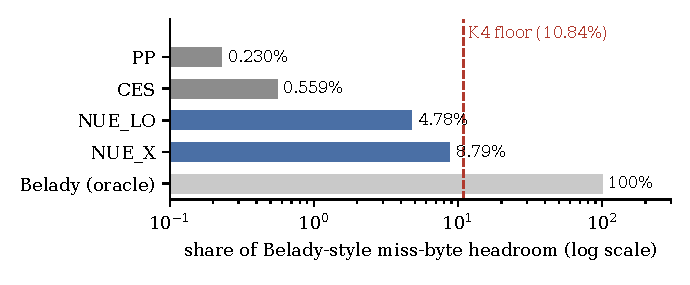
\includegraphics[width=0.78\linewidth]{figures/fig2_headroom_capture.pdf}
\caption{Share of the Belady-style miss-byte headroom captured at 1.5~GiB (log scale). The dashed line is the share that corresponds to the frozen K4 floor of 10~ms/token at $\klow$ (10.84\%). The oracle bar is clairvoyant.}
\label{fig:capture}
\end{figure}

\subsection{Prospective Viability Test}
The frozen rule K4 states that a candidate whose benefit at zero policy cost is below the success margin is infeasible regardless of any cost optimization:
\begin{equation}
V(c) < 10~\mathrm{ms/token} \;\Longrightarrow\; c \text{ infeasible}.
\label{eq:k4}
\end{equation}
Equivalently, a candidate must remove at least $10/\klow = 26.37$~MB/token of misses, 10.84\% of the oracle byte headroom.

\begin{proposition}[bounded to the tested regime]
\label{prop:main}
Under the tested Qwen3-30B-A3B-Q4\_K\_M configuration, the canonical real-runtime workload stream, the 1.5~GiB expert-memory budget, the tested demand-admission retention architecture and the frozen conversion $\klow$, the best tested causal predictive eviction policy fails the prospective economic viability criterion even assuming zero policy-computation cost.
\end{proposition}
\begin{proof}
By Eq.~\eqref{eq:value} and the frozen EVAL counters, $V(\mathrm{NUE\_X}) = 8.11$ and $V(\mathrm{NUE\_LO}) = 4.41$~ms/token, both below 10~ms/token, so K4 (Eq.~\eqref{eq:k4}) classifies both as infeasible. NUE\_X is the DEV-selected best of the tested causal predictive candidates; PP and CES capture less (Table~\ref{tab:mech}). Any non-negative policy cost lowers net value below $V$, so the conclusion holds for every realization of these policies under the frozen conversion. Both candidates therefore fail the viability test; the exact frozen classification label is listed in Appendix~\ref{app:prov}.
\end{proof}

The proposition is a statement about the tested family, conversion and regime; it is not a theorem about causal retention in general.

%=====================================================================
\section{Discussion}
\label{sec:discussion}

\subsection{Prediction Accuracy Versus Economic Value}
The results separate three conditions that predictive retention must meet, each of which failed at a different stage. \emph{Placement}: a prediction creates value only if it changes a decision whose consequence it anticipates. PP consulted its prediction during the event it predicted, so its measurable effect was intra-event self-protection, reproduced by CES without any prediction (K2). \emph{Magnitude}: placing the prediction at the future eviction decision (NUE) raised the captured headroom from 0.230\% to 8.79\%, yet the resulting gross value stayed below the floor (K4). \emph{Cost}: the measured bookkeeping cost of the realized predictor (14.59~ms/token at 1.5~GiB in the real-runtime evaluation) exceeds the replay-level gross value of every tested predictive mechanism, including NUE\_X at zero cost. A forecaster that is measurably better than trivial baselines (preceding study) can thus still be worth less than its cost as a retention controller.

\subsection{The Unresolved Oracle Gap}
The Belady-style comparator removes 40.673\% of baseline misses; NUE\_X captures 8.79\% of that byte headroom, so more than 90\% of it is not explained by any tested causal policy. The present study does not establish whether that remainder is causally recoverable. The comparator knows every future request, including requests that depend on routing many tokens ahead; some or most of its advantage may be unavailable to any causal policy, and it is not proven optimal for multi-key events. The oracle ceiling should therefore be read as an upper bound on what any policy could gain under demand admission at this budget, not as an engineering opportunity.

\subsection{Implications for MoE Memory Systems}
Two methodological lessons follow within the tested setting. First, runtime realizations of replay-validated policies need an explicit semantic-equivalence check; a 3$\times$ over-counting of policy events changed predictor dynamics, aging and cost without any visible functional error. Second, a zero-cost mechanism screen on an exact replay is cheap and informative before runtime work: the original mechanism's replay benefit at $\klow$ (0.21~ms/token, Table~\ref{tab:mech}) was about 70 times smaller than the bookkeeping cost measured in the real-runtime evaluation (14.59~ms/token), which anticipates its outcome. The present study does not show that predictive information is useless for MoE serving; it tests only retention, and it leaves untested the mechanisms in which prediction is commonly paired with proactive data movement~\cite{promoe2025,layerscope2025,expertflow2026}.

%=====================================================================
\section{Claim Boundaries and Threats to Validity}
\label{sec:threats}

\begin{table}[t]
\centering
\caption{Tested scope. Conclusions apply only within it.}
\label{tab:scope}
\small
\begin{tabularx}{\linewidth}{lX}
\toprule
Dimension & Tested \\
\midrule
Model & Qwen3-30B-A3B-Q4\_K\_M (frozen file identity) \\
Host / runtime & one Windows host (Intel Core i5-1340P); frozen modified llama.cpp runtime and expert store \\
Budget & 1.5~GiB primary; 8~GiB descriptive control; 4~GiB not used for the economic conversion \\
Workload & frozen coding workload, 512 decode tokens, seed 42, greedy; DEV selection on four development traces of the preceding study \\
Policies & \code{b\_selected}; PP and its sham; CES; NUE\_LO and NUE\_X (LEX, SOFT1, SOFT4) with demand admission \\
Predictor & \code{decayed\_transition}, decay 0.99, top-$k$ 8, horizon 1 \\
Conversion & $\klow = 0.3792$~ms/MB (two-budget association, halved) \\
\bottomrule
\end{tabularx}
\end{table}

\paragraph{Claims.} Within the scope of Table~\ref{tab:scope}, the present study shows: (1) expert usage contains predictive structure (preceding study, unchanged); (2) prediction quality alone did not imply runtime value; (3) semantic placement of policy updates mattered; (4) bookkeeping cost exceeded the retention value recovered; (5) the original mechanism captured almost none of the oracle headroom; (6) causal next-use eviction improved mechanism value substantially; (7) the best tested predictive policy captured less than 9\% of the oracle byte headroom; and (8) its conservative gross value failed the frozen floor before computation cost.

\paragraph{Not claimed.} The present study does not show that expert usage is unpredictable, that the preceding study was wrong, that all retention policies are impossible, that the oracle headroom is causally reachable, that all memory-management approaches or all predictive caching fail, or that other MoE architectures, quantizations, hardware, storage systems, budgets, prompts, predictors or caching and admission policies would behave identically.

\paragraph{Not tested.} The following were not tested and are not failures: oracle-distilled causal eviction; economic (cost-weighted) eviction; true admission or bypass; prefetch; compute/I/O overlap; scheduling; adaptive memory allocation; and general adaptive policy control.

\paragraph{Threats to validity.}
\begin{itemize}
\item \emph{Single host, model and runtime.} All timings come from one consumer machine and one model configuration; absolute costs and the cost-to-benefit ratio may differ elsewhere.
\item \emph{Limited workload diversity.} Runtime results and the EVAL stream use one workload; DEV selection used four traces of the preceding study. There is one EVAL stream and no workload-level confidence interval for the offline results.
\item \emph{Economic conversion.} $\kappa$ is a two-budget association between miss bytes and wall time, not a causal per-byte law; K4 is defined on the halved value. A different conversion could move $V$ in either direction; the classification is defined on the frozen conversion.
\item \emph{Clairvoyant comparator.} The oracle uses future information, is Belady-style for multi-key events and is not proven globally optimal; headroom shares are relative to it.
\item \emph{Replay versus runtime.} Offline replay reproduces retention mechanics exactly (Offline Replay Fidelity) but not every runtime timing effect, such as I/O contention or overlap.
\item \emph{Candidate coverage.} NUE\_X is the best of a small prospectively frozen family, not the optimal causal policy; the three NUE\_X keys were indistinguishable on DEV, so DEV evidence does not discriminate among them.
\item \emph{Scope of the negative result.} The negative result is bounded to the tested predictive family and to retention under demand admission.
\end{itemize}

%=====================================================================
\section{Related Work}
\label{sec:related}

Sparsely gated MoE layers~\cite{shazeer2017sparsely} and their large-scale variants~\cite{fedus2022switch} make expert memory placement a systems problem. Prior systems keep frequently or recently used experts resident and offload the rest~\cite{eliseev2023offloading,xue2025moeinfinity}, orchestrate CPU and GPU execution~\cite{kamahori2025fiddler}, or combine prediction with proactive caching, prefetching and scheduling~\cite{promoe2025,layerscope2025,expertflow2026}; the suitability of models for offloading has been related to local routing consistency~\cite{localroutingconsistency2025}. Offloading for single-device LLM inference more generally is studied in~\cite{sheng2023flexgen}, and~\cite{liu2026survey} surveys MoE inference optimization. Belady's study of replacement algorithms~\cite{belady1966replacement} underlies the clairvoyant comparator used here. The present study differs from these works in scope rather than mechanism: it tests one question, whether a validated routing predictor yields net runtime value when it controls retention, under prospectively frozen kill rules, and it reports a negative answer with its decomposition. Classical and learned cache-replacement policies that imitate an oracle are directly relevant to the open question of Section~\ref{sec:discussion}; their citations were not verified for this paper and are omitted rather than cited from memory.

%=====================================================================
\section{Conclusion}
\label{sec:conclusion}

Predictive structure exists in MoE expert routing, but in the tested regime it did not translate into economically useful retention control. After the runtime was made semantically equivalent to the reference and the predictor's cost was measured and attributed, the corrected predictive policy lost 15.83~ms/token at the primary budget. Offline, the original mechanism's effect was reproduced by a zero-cost shield, and the best tested causal next-use predictive policy captured 8.79\% of the clairvoyant byte headroom, worth 8.11~ms/token, below a 10~ms/token floor frozen before the test and before any computation cost. The present study is therefore closed as a negative result in the tested regime: prediction-led retention was not viable for this model, host, memory budget and workload (the exact frozen classification label is listed in Appendix~\ref{app:prov}). A separate question, outside this paper's evidence, is how much of the clairvoyant memory-management optimum can be recovered by a cheap causal policy using only information available at decision time.

\bibliographystyle{plain}
\bibliography{research3}

\appendix
\section{Provenance}
\label{app:prov}
This appendix is the only place where the repository's internal numbering is used. In that numbering the preceding study is ``Research~2'' and the present study is ``Research~3''; the reader-facing stage names used in the text map to repository identifiers as listed below. Every number in this paper is regenerated from the frozen artifacts by \code{paper/research3/scripts}; \code{SOURCE\_MAP.md} maps each claim to its stage, artifact directory and field. The closure record~\cite{argine3evidence} (directory \code{experiments/R3-final-closure/}) re-verifies the chain; the preceding-study manuscript~\cite{argine2paper} is the file \code{paper/research2/manuscript.tex}. The frozen coding workload has repository identifier \code{r2-11-coding-v1}.

\begin{table}[h]
\centering
\caption{Present study: reader-facing stage, repository identifier, commit and freeze (SHA-256).}
\label{tab:prov}
\small
\begin{tabularx}{\linewidth}{>{\raggedright\arraybackslash}p{0.34\linewidth}ll>{\raggedright\arraybackslash}X}
\toprule
Reader-facing name & Repository ID & Commit & Freeze (SHA-256) \\
\midrule
Runtime Semantic Equivalence & R3-03A & \code{3c37870} & FREEZE.json file \hsh{0ebcd1354e3bd1d1454bce056fc0cd7430ea8997d33e8e9ed6134d1e3a632cc5} \\
Predictor Cost Attribution (microbenchmark) & R3-03B & \code{757ddfe} & \hsh{abb451010b04782a56c51420485908871e1a77e87dd18b22f75b5e0580dd7009} \\
Predictor Cost Attribution (end to end) & R3-03B & \code{46cab36} & \hsh{1846b00954e033bc9a4cb136cd05373a411d7a8de699923235f31dbfd2f53448} \\
Real-Runtime Retention Evaluation (evidence) & R3-04 & \code{0f72427} & \hsh{71fca58e65853c325ba7622d7565e51be85a54f46394de8d4f4ee2e0753adfa2} \\
Real-Runtime Retention Evaluation (closure) & R3-04 & \code{91aa9b4} & CLOSURE.json file \hsh{24a09785677bb1fba029cd5303aef630f1dc57d46571f0b858acb162b947555a} \\
Prospective Predictive-Retention Falsification (protocol) & R3-05 Phase 0 & \code{402cf6a} & \hsh{415f78a850a2917a2457797106589433f944c07a863f80b14cef88fde6232ae3} \\
Offline Replay Fidelity & R3-05 R1 & \code{12e3347} & \hsh{8d025fdfb3d2a48c54e4d905f3a0e3aad2dd70ed9fdabf602b21ec2b600c3382} \\
Clairvoyant Retention Headroom & R3-05 R2 & \code{fc8e631} & \hsh{8b22e41505e3c14b78b6c924b703f1da4b26643123a9240f7bd9ad7d232afa44} \\
Current-Event Shielding & R3-05 R3 & \code{f6e7780} & \hsh{1993adfa510bc792878fadf26ff3044fb5d7cc1c88d8ab37211271c19266e7b6} \\
Causal Next-Use Eviction & R3-05 R4 & \code{6129007} & \hsh{3f52a06eeec6f581be8d0659071b0de0dc9412849de3d10b6bd175cf8231b478} \\
Present-study closure & Research~3 closure & \code{3aa389e} & \hsh{760a22d69abdd207c7ecd4b4f1012b85711b20aa3cb623cddb55d0c8802a5717} \\
\bottomrule
\end{tabularx}
\end{table}

\begin{table}[h]
\centering
\caption{Exact frozen classification labels behind the reader-facing outcomes of Table~\ref{tab:stages}. The labels are unchanged from the frozen evidence.}
\label{tab:labels}
\small
\begin{tabularx}{\linewidth}{>{\raggedright\arraybackslash}p{0.30\linewidth}X}
\toprule
Reader-facing stage & Frozen label \\
\midrule
Runtime Semantic Equivalence & \code{R3\_03A\_RUNTIME\_SEMANTIC\_CONFORMANCE\_PASS} \\
Predictor Cost Attribution & \code{R3\_03B\_EXPLAINED} \\
Real-Runtime Retention Evaluation & \code{R3\_04\_CLOSED\_NET\_LOSS} \\
Offline Replay Fidelity & \code{R3\_05\_R1\_FIDELITY\_PASS} \\
Clairvoyant Retention Headroom & \code{R3\_05\_K1\_HEADROOM\_PASS} \\
Current-Event Shielding & \code{R3\_05\_K2\_RETIRE\_CURRENT\_PP} \\
Causal Next-Use Eviction (and falsification sequence) & \code{R3\_05\_PREDICTIVE\_RETENTION\_KILLED} \\
Overall & \code{R3\_CLOSED\_NEGATIVE\_PREDICTIVE\_RETENTION\_NOT\_VIABLE\_IN\_TESTED\_REGIME} \\
\bottomrule
\end{tabularx}
\end{table}

\begin{table}[h]
\centering
\caption{Preceding study: reader-facing stage (numbering of Table~\ref{tab:prev}) and repository identifier. The repository identifiers are not renumbered.}
\label{tab:prevprov}
\small
\begin{tabularx}{\linewidth}{r>{\raggedright\arraybackslash}Xl}
\toprule
 & Reader-facing name & Repository ID \\
\midrule
1 & Oracle Trace Contract and Replay Validation & R2-01 \\
2 & Oracle vs Retention Baselines & R2-02 \\
3 & Expert-Memory Budget Sensitivity & R2-03 \\
4 & Recoverable-Margin Analysis & R2-04 \\
5 & Expert Frequency and Concentration & R2-05 \\
6 & Routing Transition Structure & R2-06 \\
7 & Reuse Distance and Working-Set Structure & R2-07 \\
8 & Routing Drift and Workload Dependence & R2-08 \\
9 & Prediction Benchmark & R2-09 (sub-phases R2-09A, R2-09B) \\
10 & Causal Working-Set Predictor & R2-10 \\
11 & Retention Feasibility Bridge & R2-BRIDGE-01 \\
12 & Prediction-Driven Retention & R2-11 \\
13 & Real-Runtime Decode Throughput & R2-12 \\
\bottomrule
\end{tabularx}
\end{table}

\end{document}
